\chapter{Complex Plane}
This chapter covers the basic geometry and topology of the complex plane, including the equations of lines and circles, extended complex plane which includes the Riemann sphere and stereographic projection, Mobius transformations acting on the extended complex plane, Mobius transformations take circlines to circlines.

\section{Review of Complex Numbers}
The imaginary unit $i$ has the property $i^2=-1$. A complex number is of the form $z=a+bi$, where $a,b\in\RR$; we call $a$ the real part of $z$, denoted by $a=\Re(z)$, and $b$ is the imaginary part of $z$, denoted by $b=\Im(z)$. Two complex numbers are equal if and only they have the same real part and the same imaginary part.

We define addition as summing up the real and imaginary parts respectively:
\[(a+bi)+(c+di)=(a+c)+(b+d)i.\]
Multiplication is defined as
\[(a+bi)(c+di)=(ac-bd)+(ad+bc)i\]
where we have made use of the relation $i^2=-1$. Before discussing division, we define 

\section{Geometric Representation of Complex Numbers}

\section{$\CC$ As Metric Space}
We can identify $\CC$ with the plane $\RR^2$ by taking
real and imaginary parts. Thus we have mutually inverse bijections
\[z\mapsto(\Re z,\Im z)\]
from $\CC$ to $\RR^2$, and
\[(x,y)\mapsto x+iy\]
from $\RR^2$ to $\CC$. As we have seen, $\RR^2$ is a metric space with the metric induced from the Euclidean norm
\[\norm{(x,y)}_2=\sqrt{x^2+y^2}.\]
This gives a metric on $\CC$ by the identification $\CC\cong\RR^2$ described above.

If $z=\Re z+i\Im z$ is a complex number we write $|z|$ (called the \vocab{modulus}) for this Euclidean norm; that is,
\[|z|=\sqrt{(\Re z)^2+(\Im z)^2}.\]
The distance between the two points $z,w\in\CC$ is then $|z-w|$.

Let us write down some basic properties of the modulus $|z|$. Recall that $e^{i\theta}=\cos\theta+i\sin\theta$ when $\theta\in\RR$. For now, we will take this as the definition of $e^{i\theta}$. Later on we will define the complex exponential function $e^z$ and link the two concepts.

\begin{lemma}
Let $z,w\in\CC$. Then
\begin{enumerate}[label=(\arabic*)]
\item $|z|^2=z\bar{z}$, where $\bar{z}$ is the complex conjugate of $z$;
\item If $z=re^{i\theta}$, where $r\in[0,\infty)$ and $\theta]in\RR$, then $|z|=r$;
\item $|zw| = |z||w|$.
\end{enumerate}
\end{lemma}

\begin{proof} \
\begin{enumerate}[label=(\arabic*)]
\item If $z=a+ib$ then $z\bar{z}=(a+ib)(a-ib)=a^2+b^2$.
\item We have $z=r\cos\theta+ir\sin\theta$ and so
\[|z|=\sqrt{r^2\cos^2\theta+r^2\sin^2\theta}=r.\]
\item One can calculate directly, writing $z=a+ib$ and $w=c+id$. Alternatively, write $z=re^{i\theta}$, $w=r^\prime e^{i\alpha}$, and then observe that $zw=rr^\prime e^{i(\theta+\alpha)}$ and use (2).
\end{enumerate}
\end{proof}

\section{Topology of $\CC$}
One can make sense of the notion of open set, closure, interior and so on by identifying $\CC$ with $\RR^2$.

\begin{definition}
$U\subset\CC$ being \vocab{open} means that if $z\in U$ then some ball $B_r(z)$, $r>0$, also lies in $U$, where
\[B_r(z)\coloneqq\{w\in\CC\mid|z-w|<r\}.\]
\end{definition}

In complex analysis it is often convenient to work with connected open sets, and these are called domains.

\begin{definition}
A connected open subset $D\subseteq\CC$ of the complex plane will be called a domain.
\end{definition}

We have seen that for open subsets of normed spaces (such as $\RR^2$ with the Euclidean metric), the notions of connectedness and path-connectedness are the same thing. Therefore domains are always path-connected.

\section{Geometry of $\CC$}
Let us take a closer look at the geometry of the complex plane in terms of the distance $|z-w|$. When we talk about lines and circles in $\CC$, we mean sets that are lines and circles in $\RR^2$ (under the identification of $\RR^2$ with $\CC$).

\begin{lemma}[Lines]
Let $a,b\in\CC$ be distinct complex numbers. Then the set $\{z\in\CC\mid|z-a|=|z-b|\}$ is a line. Conversely, every line can be written in this form.
\end{lemma}

\begin{proof}
Given $a$ and $b$, the set of $z$ such that $|z-a|=|z-b|$ is the set of points equidistant from $a$ and $b$, which is the perpendicular bisector of the line segment $\overline{ab}$. Conversely, every line is the perpendicular bisector of some line segment.
\end{proof}

\begin{remark}
Sometimes, the set of all complex numbers satisfying some given equation is called a \vocab{locus}. Thus the locus of complex numbers satisfying $|z-a|=|z-b|$ is a line. The representation of lines in the above form is very much non-unique: for example, the $x$-axis (the set of $z$ with zero imaginary part) can be described as $\{z\mid|z-a|=|z-\bar{a}\}$ for any complex number $a$.
\end{remark}

Now we turn to circles. Evidently, the set $\{z\in\CC\mid|z-c|=r\}$, where $c\in\CC$ and $r\in(0,\infty)$, is a circle centred on $c$ and with radius $r$. Conversely, every circle can be written in this form. Less obvious is the following.

\begin{lemma}[Circles]
Let $a,b\in\CC$ be distinct complex numbers, and let $\lambda\in(0,\infty)$, $\lambda\neq1$. Then the locus of complex numbers satisfying $|z-a|=\lambda|z-b|$ is a circle. Conversely, every circle can be written in this form.
\end{lemma}

\begin{proof}
Without loss of generality, $b=0$ (a translate of a circle is a circle). Now observe the identity
\[|tz+a|^2=t(t+1)|z|^2-t|z-a|^2+(t+1)|a|^2,\]
valid for all $a,z\in\CC$ and all $t\in\RR$. This can be checked by a slightly tedious calculation. Applying it with $t=\lambda^2-1$ gives
\[|(\lambda^2-1)z+a|=\lambda|a|,\]
which is clearly the equation of a circle. Taking $a=-c(\lambda^2-1)$ and $\lambda=\frac{r}{|c|}$, this gives $|z-c|=r$, and so every circle can be written in this form.
\end{proof}

\begin{remark}
This lemma is an interesting and non-obvious fact in classical Eu-
clidean geometry. Phrased in that language, if $A$, $B$ are points in the plane, and if $\lambda\in(0,\infty)$, $\lambda\neq1$, then the set of all points $P$ such that $\frac{|PA|}{|PB|}=\lambda$ is a circle. We have just proven that this is true using complex numbers.
\end{remark}

\section{Extended Complex Plane $\CC_\infty$}
\subsection{Stereographic projection}
Let
\[\SSS=\{(x,y,z)\in\RR^3\mid x^2+y^2+z^2=1\}\]
be the unit sphere of radius $1$ centred at the origin in $\RR^3$. View the complex plane $\CC$ as the copy of $\RR^2$ inside $\RR^3$ given by the plane $\{(x,y,0)\in\RR\mid x,y\in\RR\}$. Thus $z=x+iy$ corresponds to the point $(x,y,0)$. Let $N$ be the ``north pole'' $N=(0,0,1)$ of $\SSS$.

We can define a bijective map $S:\CC\to\SSS\setminus\{N\}$ as follows. To determine $S(z)$, join $z$ to $N$ by a straight line, and let $S(z)$ be the point where this line meets the sphere $\SSS$. This map (or more accurately its inverse) is called \vocab{stereographic projection}.

It is not too hard to give an explicit formula for $S(z)$.

\begin{lemma}
Suppose that $z=x+iy$. Then
\[S(z)=\brac{\frac{2x}{x^2+y^2+1},\frac{2y}{x^2+y^2+1},\frac{x^2+y^2-1}{x^2+y^2+1}}.\]
\end{lemma}

\begin{proof}
The general point on the line joining $z$ and $N$ is $t(0,0,1)+(1-t)(x,y,0)$. There is a unique value of $t$ for which this point lies on the sphere, namely $t=\frac{x^2+y^2-1}{x^2+y^2+1}$, as can be easily checked.
\end{proof}

\begin{figure}[H]
\centering
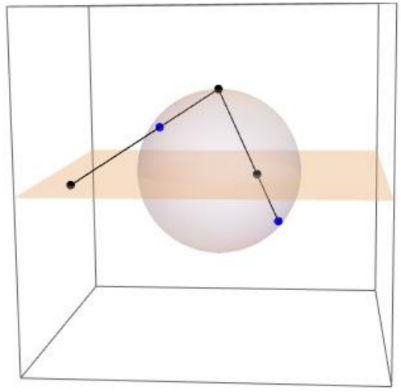
\includegraphics[width=0.5\linewidth]{images/stereographic-projection-map.png}
\caption{The stereographic projection map}
\end{figure}

We remark that the same formula can be written in the alternative form
\[S(z)=\frac{1}{1+|z|^2}\brac{2\Re(z),2\Im(z),|z|^2-1}.\]
As we have seen, $\CC$ may be identified with $\SSS\setminus\{N\}$ by stereographic projection. The set $\SSS\setminus\{N\}$ has a natural metric, namely the one induced from the Euclidean metric on $\RR^3$. This induces a metric $d$ on $\CC$, the unique metric on $\CC$ such that $\SSS$ is an isometry. To spell it out,
\[d(z,w)\coloneqq\norm{S(z)-S(w)}.\]
Here is a formula for this metric.
\begin{lemma}
For any $z,w\in\CC$ we have
\[d(z,w)=\frac{2|z-w|}{\sqrt{1+|z|^2}\sqrt{1+|w|^2}}.\]
\end{lemma}

\begin{proof}
Since $\norm{S(z)}=\norm{S(w)}=1$ we have $\norm{S(z)-S(w)}^2=2-2\langle S(z),S(w)\rangle$, where $\langle,\rangle$ is the usual Euclidean inner product on $\RR^3$. Using the formulae (and after a little computation),
\[\langle S(z),S(w)\rangle=1-\frac{2|z-w|^2}{(1+|z|^2)(1+|w|^2)}.\]
Therefore
\[\norm{S(z)-S(w)}^2=\frac{4|z-w|^2}{(1+|z|^2)(1+|w|^2)}\]
as required.
\end{proof}

\subsection{Adding in $\infty$}
Now it is time to add in the point at infinity, which we will call $\infty$ (note this is just a symbol).

Now (exercise) as $|z|\to\infty$, $S(z)\to N$. Therefore, once we have identified $\CC$ with $\SSS\setminus\{N\}$, it is natural to identify $\infty$ with $N$, and hence $\CC_\infty=\CC\cup\{\infty\}$ with the whole sphere $\SSS$. We extend the map $S$ to a map $S:\CC_\infty\to\SSS$ by defining $S(\infty)=N$.

Using, once again, the Euclidean metric on $S$, we can extend $d$ to a metric on $\CC_\infty$, the unique metric for which the map $S$ is an isometry.

\begin{lemma}
For any $z\in\CC$ we have
\[d(z,\infty)=\frac{2}{\sqrt{1+|z|^2}}.\]
\end{lemma}

\begin{proof}
By definition, $d(z,\infty)=\norm{S(z)-S(\infty)}=\norm{S(z)-N}$, where $N$ is the north pole on the sphere. We may now proceed in much the same way as before, except the calculation is easier this time. The details are left as an exercise.
\end{proof}

We turn now to a few examples, which show that adding $\infty$ to $\CC$ in this way leads to a space with nice analytic properties.

\begin{example}[Translations]
Let $a\in\CC$. Define $f:\CC_\infty\to\CC_\infty$ by $f(z)=z+a$ for $z\in\CC$ and $f(\infty)=\infty$. Then $f$ is a continuous bijection.
\end{example}

\begin{proof}
Clearly $f$ is continuous with respect to the usual metric on $\CC$. Therefore, restricted to $\CC$, it is also continuous with respect to $d$, since $d$ is equivalent to the usual metric.

It remains to check continuity at $\infty$. Let $\epsilon>0$. Now if $\delta>0$ and if $d(z,\infty)<\delta$ then $|z|>\sqrt{\frac{4}{\delta^2}-1}$ and so $|f(z)|>\sqrt{\frac{4}{\delta^2}-1}-|a|$. This tends to $\infty$ as $\delta\to0$, so by choosing $\delta$ small enough in terms of $\epsilon$ it will follows that
\[d\brac{f(z),\infty}=\frac{2}{\sqrt{1+|f(z)|^2}}<\epsilon.\]
\end{proof}

\begin{example}[Dilations]
Let $b\in\CC$. Define $f:\CC_\infty\to\CC_\infty$ by $f(z)=bz$ for $z\in\CC$ and $f(\infty)=\infty$. Then $f$ is a continuous bijection.
\end{example}

\begin{proof}
This is very similar to the argument for translations and we leave the details as an exercise.
\end{proof}

The final example is the most interesting one.

\begin{example}[Inversion]
Define $f:\CC_\infty\to\CC_\infty$ by $f(z)=\frac{1}{z}$ for $z\in\CC\setminus\{0\}$, $f(0)=\infty$ and $f(\infty)=0$. Then $f$ is a continuous bijection.
\end{example}

\begin{proof}
As before, the equivalence of $d$ and the usual metric on $\CC$ means that $f$ is continuous except possibly at $0$ and $\infty$.

We prove that $f$ is continuous at $0$, leaving the continuity at $\infty$ as an exercise (similar to the example on translations).

Let $\epsilon>0$ be small. Then there is $\delta$ such that $\frac{2t}{\sqrt{1+t^2}}\le\epsilon$ for all $t\in[0,\delta]$. If $|z|<\delta$ then
\[d\brac{f(z),f(0)}=d\brac{\frac{1}{z},\infty}=\frac{2}{\sqrt{1+\frac{1}{|z|^2}}}=\frac{2|z|}{\sqrt{1+|z|^2}}\le\epsilon.\]
This indeed shows that $f$ is continuous at $0$.
\end{proof}

\subsection{M\"{o}bius maps}
In this subsection and subsequent ones we look at an important class of maps from $\CC_\infty$ to itself, the M\"{o}bius maps.

\subsection{The complex projective line $\PP^1(\CC)$}
\subsection{Decomposing M\"{o}bius maps}
\subsection{Basic geometry of M\"{o}bius maps}